\documentclass[12pt]{article}
\usepackage{graphicx}
\usepackage[utf8]{inputenc}
\usepackage{amsmath}
\usepackage{biblatex}
\addbibresource{kaynakca.bib}
\usepackage{amsfonts}
\usepackage{amssymb}
\usepackage{mathtools}
\usepackage{physics}
\usepackage{siunitx}
\usepackage{unicode-math}
\usepackage{subcaption}
\usepackage{xcolor}
\usepackage{listings}
\usepackage{tikz}
\usetikzlibrary{shapes.geometric, arrows}
\usepackage{booktabs}
\usepackage{geometry}
\usepackage{adjustbox}
\usepackage{fancybox}
\usepackage{lipsum}
\usepackage{enumitem}
\usepackage{rotating}
\usepackage{longtable}
\usepackage{multirow}
\usepackage{geometry}
\usepackage{graphicx}
\usepackage{array}
\usepackage{booktabs}
\usepackage{caption}
\geometry{a4paper, margin=1in}


\definecolor{codeblue}{RGB}{0,0,255}

\lstset{
    basicstyle=\small\itshape\color{codeblue},
    language=Python,
    breaklines=true
}
\renewcommand{\refname}{Kaynakça}
\renewcommand{\contentsname}{İçindekiler Tablosu}
\renewcommand{\figurename}{Şekil}

\begin{document}

\begin{figure}
    \centering
    
\includegraphics[width=3\textwidth, height=5cm, keepaspectratio]{ksbu.png}
    \label{fig:enter-label}
\end{figure}

\title{Hair GAN's}
\author{Halime Rüya SARIKAYA}
\date{14.06.2024}

\maketitle
\newpage
\tableofcontents
\newpage
\begin{center}
    
\end{center}

\section{Özet}

Generative Adversarial Networks (GAN'lar), son yıllarda yapay zeka araştırmalarında büyük ilgi gören ve başarılarıyla dikkat çeken bir modeldir. GAN'lar, iki temel bileşenden oluşan bir yapay sinir ağı mimarisine dayanır: bir üretici (generator) ve bir ayırt edici (discriminator). Bu iki bileşen arasında rekabet oluşturularak, üreticinin gerçekçi görüntüler üretmesi ve ayırt edicinin bu görüntüleri gerçek verilerden ayırt etme yeteneğini geliştirmesi sağlanır.
\\
Üretici ağ, rastgele gürültüden başlayarak gerçekçi veri üretmeye çalışırken, ayırt edici ağ, üretilen verilerin gerçek verilerden ayırt edilmesini sağlamak için eğitilir. Bu süreçte, iki ağ arasındaki rekabet, üretici ağın giderek daha gerçekçi veriler üretmesini ve ayırt edici ağın daha hassas hale gelmesini sağlar. Sonuç olarak, GAN'lar son derece gerçekçi verilerin üretilmesine olanak tanır.GAN'lar birçok alanda kullanılabilir:

\begin{table}[htbp]
\centering
\captionsetup{justification=centering}
\caption{GAN'ların Kullanım Alanları ve Özellikleri}
\label{tab:gan-kullanim}
\begin{tabular}{|p{4.5cm}|p{9cm}|}
\hline
\textbf{Kullanım Alanı} & \textbf{Özellikleri} \\
\hline
Görüntü Üretimi ve Düzeltme & GAN'lar, yüksek çözünürlüklü ve gerçekçi görüntülerin üretilmesi ve eksik veya bozuk görüntülerin düzeltilmesi için kullanılabilir. Özellikle, sanat eserlerinin veya fotoğrafların yeniden oluşturulması ve iyileştirilmesi için kullanılabilirler. \\
\hline
Stil Transferi & GAN'lar, farklı sanat tarzları veya görüntü stillerinin birleştirilmesi veya aktarılması için kullanılabilir. Bu, bir resmin tarzının başka bir resme uygulanmasını sağlayarak, yeni ve yaratıcı görsellerin oluşturulmasına olanak tanır. \\
\hline
Veri Artırma & Sınırlı sayıda veri örneğiyle çalışıldığında, GAN'lar yeni ve çeşitli veri örneklerinin sentezlenmesi için kullanılabilir. Bu, modelin daha genelleme yeteneğini artırabilir ve eğitim verisi eksikliği durumunda performansı artırabilir. \\
\hline
Oyun ve Animasyon & GAN'lar, karakter ve sahne oluşturmak için oyun ve animasyon endüstrisinde kullanılabilir. Karakterlerin ve sahnelerin gerçekçi ve etkileyici olmasını sağlar, bu da oyunların ve animasyonların daha çekici olmasını sağlar. \\
\hline
\end{tabular}
\end{table}
Projede, özellikle yüz ve saç stilleri oluşturma üzerine odaklanarak, GAN'ların yaratıcı içeriklerin oluşturulmasındaki potansiyelini ortaya koymayı amaçlanmaktadır. Bu amaç doğrultusunda, GAN'lar üzerinde deneyler yapılacak, eğitim süreçlerini optimize edilecek ve gerçekçi görünümlü yüz ve saç stilleri üretmeye odaklanılacaktır.
\newpage
\section{Anahtar Kelimeler}

\begin{table}[htbp]
\centering
\begin{tabular}{|p{1.0\linewidth}|}
\hline
\textbf{Anahtar Kelimeler} \\
\hline
GAN (Generative Adversarial Networks) \\
Yüz sentezi \\
Saç stil üretimi \\
Derin öğrenme \\
Yapay zeka \\
Görüntü sentezi \\
Veri artırma \\
Sanat ve yaratıcılık \\
Görüntü oluşturma \\
Görüntü işleme \\
Veri sentezi \\
Yapay sinir ağları \\
Görüntü üretimi \\
Yaratıcı içerik oluşturma \\
Görüntü analizi \\
Derin öğrenme modeli \\
Sentetik veri oluşturma \\
Yüz tanıma \\
Görüntü gerçekçiliği \\
Yapay zeka eğitimi \\
Yapay veri üretimi \\
Görüntü manipülasyonu \\
Görüntü kalitesi \\
Veri çeşitliliği \\
Sanal insan oluşturma \\
Görüntü yeniden oluşturma \\
Yapay zeka sanatı \\
Görüntü sentezi teknikleri \\
Yüz modelleme \\
Görüntü tabanlı öğrenme \\
\hline
\end{tabular}
\caption{Yapay Zeka Projesi Anahtar Kelimeler}
\label{tab:anahtar-kelimeler}
\end{table}
\section{Metodoloji}
Bu bölümde, projenin tasarımı ve uygulanmasıyla ilgili detaylı bir açıklama sunulacaktır. Proje başlangıcından sonuna kadar izlediğimiz yöntemleri ve kullanılan araçları açıklayarak, projenin nasıl yapılandırıldığını ve uygulandığını detaylı bir şekilde ortaya koyulacaktır.
Projenin temel amacı, GAN (Generative Adversarial Networks) teknolojisinin kullanılarak yaratıcı içeriklerin üretilmesidir. Bu amaç doğrultusunda, öncelikle mevcut bir StyleGAN projesi üzerinde çalışmaya başlanmıştır.Bu projeyi, NVIDIA'nın resmi StyleGAN kodu ve diğer açık kaynaklı kaynaklar temel alınarak uyarlamaya çalışılmıştır.\cite{Azmarie}
Uyarlamaya çalışırken, projenin özgün amacını koruyarak, StyleGAN'ın mimarisini anlamaya ve geliştirmeye odaklanılmıştır. Özellikle, modelin yapısını anlamak, eğitim veri kümesini hazırlamak ve eğitim sürecini başlatmak için gerekli adımlar izlenmiştir. Bu süreçte, kullanılan veri kümesinin seçimi ve hazırlanması, modelin mimarisinin yapılandırılması ve eğitim sürecinin izlenmesi gibi adımlar önem taşımaktadır.
Hazır bir StyleGAN projesi üstünde çalışma yaparken yaşanılan en büyük zorluk kütüphane sürümlerinin uyuşmazlığından kaynaklanmıştır . Bu sebeple kütüphane araştırmaları yapılmıştır . Hazır bir StyleGAN projesinden olumlu sonuç alınamamış olup kendi model eğitimimize geçilmiştir.Model eğitimi yaparken en büyük zorluk ise oluşan görüntü kalitesinin istenilen şekilde olmamasıdır.Kaliteli görüntüler üretmek için yapılan düzeltmeler ve araştırmalara bu bölümde yer verilmiştir.
\subsection{Tensorflow Nedir?}
TensorFlow, Google tarafından geliştirilen ve derin öğrenme ve makine öğrenimi için açık kaynaklı bir kütüphanedir. Temelde büyük sayısal hesaplamaları gerçekleştirmek için kullanılan bir açık kaynaklı yazılım kütüphanesi olan NumPy’a benzerdir, ancak TensorFlow, hesaplamaları GPU ve TPU gibi farklı donanım kaynaklarında dağıtmak için optimize edilmiştir. TensorFlow, derin öğrenme modelleri oluşturmak, eğitmek ve dağıtmak için kapsamlı bir araç seti sunar. Grafik tabanlı bir hesaplama modeli kullanarak, veri akışının hesaplanması için bir hesaplama grafiği oluşturur ve bu grafiği TensorFlow’un yürütme motoru üzerinden çalıştırır. Bu, paralel işlem gücünden yararlanarak büyük ölçekte karmaşık hesaplamaları gerçekleştirebilir. TensorFlow, tensorler adı verilen veri yapısı etrafında döner. Bu tensorler, bir işlemden bir işleme akarak ilerler.0 boyutlu tensore scaler , 1 boyutlu tensore vektör , 2 boyutlu tensore matris denir Genel olarak tensor n boyutlu dizilerdir.
\begin{figure}[h]
    \centering
    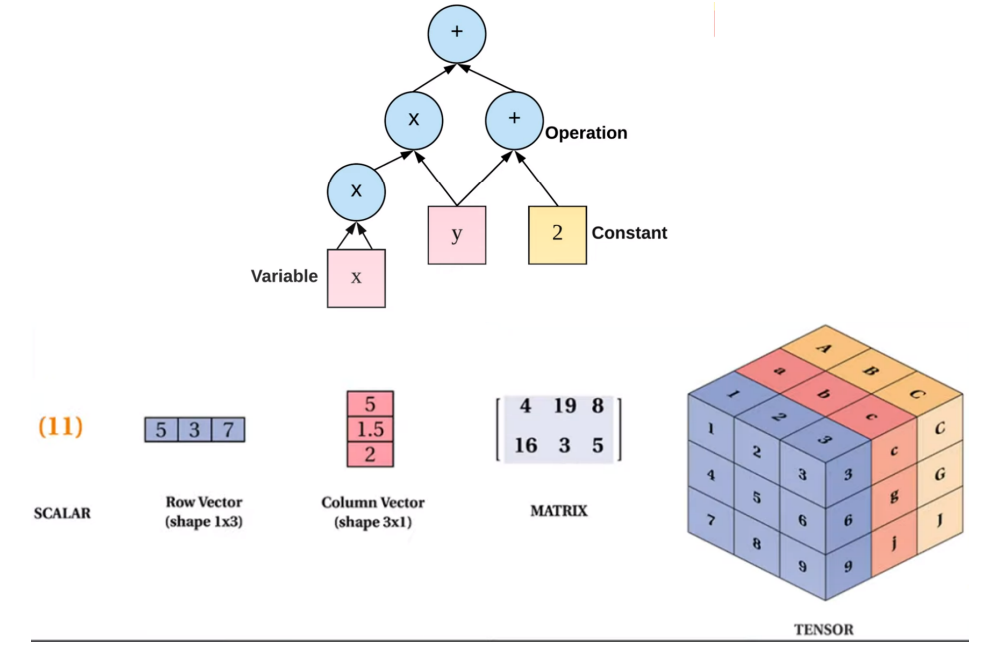
\includegraphics[width=5\textwidth, height=5cm, keepaspectratio]{tensor.png}
    \label{fig:enter-label}
\end{figure}
\subsection{Raw Images & Alıgned Images (Ham ve Hizalanmış Görüntü)}
Ham görüntü,bir sensör tarafından doğrudan yakalanan ve işlenmemiş olan orijinal görüntüdür. Ham görüntü, genellikle sensör tarafından algılanan ışık yoğunluğu ve renk bilgisini içerir. Her pikselin sensör tarafından kaydedilen doğrudan değerlerini temsil eder. Bu nedenle, renk dengesi, pozlama ve diğer görüntü özellikleri genellikle işlenmemiştir.
Hizalanmış görüntü, genellikle bir kaynak noktasına veya referans noktasına göre hizalanmış olan bir görüntüdür. Hizalama işlemi, farklı görüntüler arasındaki konumsal farklılıkları veya dönüşümleri düzeltmek için yapılır.
\begin{figure}[h]
    \centering
    \begin{minipage}{0.45\textwidth}
        \centering
        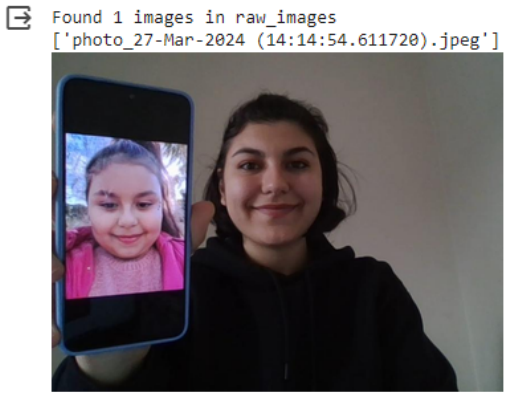
\includegraphics[width=\textwidth]{raw.png} 
        \caption{Ham görüntü örneği}
        \label{fig:resim1}
    \end{minipage}\hfill
    \begin{minipage}{0.45\textwidth}
        \centering
        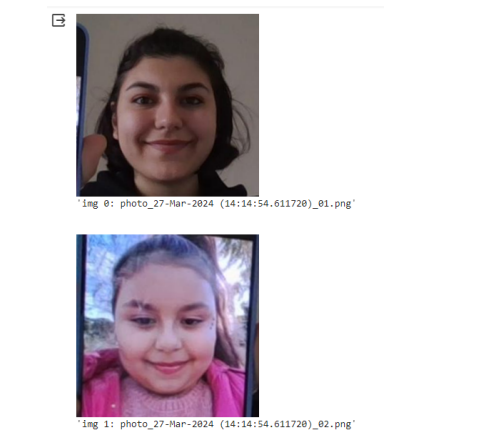
\includegraphics[width=\textwidth]{aligned.png}
        \caption{Hizalannmış görüntü örneği}
        \label{fig:resim2}
    \end{minipage}
\end{figure}
\subsection{Hızlı ve Yavaş Versiyon}
Hızlı sürüm, aynı işlevi yerine getiren ancak daha hızlı çalışan ve daha az kaynak tüketen bir versiyondur. Genellikle daha az hesaplama yapılır veya daha az veri işlenirken kullanılır. Hızlı sürüm, daha az doğruluk gerektiren veya daha basit problemleri çözmek için tercih edilebilir.Yavaş sürüm, bir yazılım veya algoritmanın daha uzun sürede çalışan ve daha fazla kaynak tüketen bir versiyonudur. Genellikle daha ayrıntılı hesaplamalar yapılır veya daha fazla veri işlenirken kullanılır. Yavaş sürüm, daha doğru sonuçlar elde etmek veya daha karmaşık problemleri çözmek için tercih edilebilir.
\subsection{Optimizasyon Algoritmaları}
\subsubsection{Optimizasyon Nedir?}
Yapay sinir ağlarında uygulanan aşamalardan olan optimizasyon için öncelikle hata fonksiyonunun (loss function) tanımlanmasına ihtiyaç duyulmaktadır. Geleneksel ve modern yöntemlerde, optimizasyon demek, bir maliyet/kayıp fonksiyonunun belirli kısıtlara ve parametrelere tabi olarak en yüksek/düşük hale getirilmesi demektir. Yapılan optimizasyon neticesinde bulunan minimum değerin, lokal minima değil, global minimaya götürmesi, optimizasyonun en önemli hedefidir. Eğitim setinde bulunan minimum değerler, en iyi sonucun bulunduğunu garanti etmez; optimizasyon, lokal minima ya da düşmüş de olabilir. Bu yüzden hangi modelde hangi optimizasyonun uygulandığı önem kazanır.\cite{Seyyarer2020}
\begin{figure}[h]
    \centering
    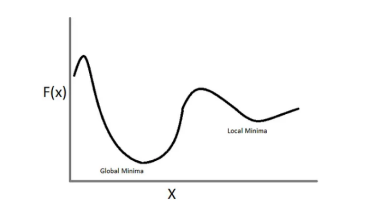
\includegraphics[width=8\textwidth, height=8cm, keepaspectratio]{opt1.png}
    \label{fig:enter-label}
\end{figure}
\subsubsection{Momentum Algoritması}
Momentum, gradyan tabanlı optimizasyon algoritmalarında kullanılan bir tekniktir. Bu teknik, gradyanın yönüne ve büyüklüğüne bağlı olarak bir hız terimi ekleyerek güncellemeleri hızlandırır. Örneğin, bir topun yokuş aşağı yuvarlanırken kazandığı momentumu düşünebilirsiniz. Her adımda, topun hızı, önceki adımlardaki hızı ve güncel gradyanın yönüne bağlı olarak belirlenir. Bu sayede, top daha hızlı aşağıya doğru hareket eder. Aynı şekilde, momentum terimi gradyan tabanlı optimizasyonlarda da benzer bir işlev görür.

Momentum, özellikle yerel minimumlardan kaçınmak ve daha hızlı yakınsamak için faydalı olabilir. Ancak, çok büyük bir momentum değeri modelin istenmeyen şekilde sıçramasına neden olabilir.
\subsubsection{RMSProp (Root Mean Square Propagation)Algoritması}
RMSProp, öğrenme oranını her parametre için ayrı ayrı ayarlayarak adaptif bir şekilde günceller. Bu sayede, nadir görülen özelliklere sahip parametrelerin daha hızlı güncellenmesi sağlanır. RMSProp'un ana fikri, gradyanların değişim hızını izlemektir. Yani, büyük değişim hızına sahip parametrelerin öğrenme oranı küçültülürken, küçük değişim hızına sahip parametrelerin öğrenme oranı büyütülür. Bu, modelin daha dengeli bir şekilde güncellenmesini sağlar ve daha hızlı yakınsamasına yardımcı olabilir.
\subsubsection{ADAM (Adaptive Moment Estimation )Algoritması}
2015 yılında Toronto Üniversitesi'nde sunulan Adam optimizasyon algoritması; Momentum ve RMSprop algoritmalarını birleştirerek kullanılan bir algoritmadır. Adam algoritması, son zamanlarda doğal dil işleme konularında geniş kabul görmüştür. Bu algoritma, derin öğrenme alanında çok kullanılmaktadır, çünkü iyi sonuçları hızlı bir şekilde vermektedir.

Momentum ve RMSProp algoritmaları, başlangıç değeri olarak sıfırdan başlamakta ve bu hız bakımından algoritmaları dezavantajlı duruma getirmekteydi. RMSProp ve Momentum algoritmalarında doğrudan türev uygulanarak yönlendirme yapılırken, Adam algoritmasında önce iterasyon sayısına bağlı bir düzeltme yapılır. Bu düzeltme, algoritmanın başlangıçta daha iyi performans göstermesine yardımcı olur.
\begin{equation}\cite{OpenAI}
\theta_{t+1} = \theta_{t} - \frac{\alpha}{\sqrt{v_t} + \epsilon} \cdot m_t
\end{equation}

Burada:
\begin{itemize}
    \item $\theta_{t}$, t anındaki parametre vektörü,
    \item $m_t$, momentum vektörü,
    \item $v_t$, RMSProp'tan gelen hareketli ortalama karesi,
    \item $\alpha$, öğrenme oranı,
    \item $\epsilon$, stabilizasyon terimi (genellikle çok küçük bir değer, örneğin $10^{-8}$).
\end{itemize}
\textbf{ADAM Algoritmasının Avantajları}
\begin{itemize}
    \item Algoritmanın uygulaması kolaydır.
    \item Küçük hafıza gereksinimlerine ihtiyaç duyar.
    \item Gürültülü veri setleri için uygundur. 
\end{itemize}
\subsection{DnnLib Kütüphanesi}
DNNLIB, NVIDIA'nın Derin Öğrenme Uygulamaları için Kütüphane (Deep Learning Applications Library) olarak bilinen bir kütüphanedir. Bu kütüphane, genellikle stilize edilmiş GAN modelleri gibi yenilikçi derin öğrenme tekniklerini uygulamak için kullanılır.
DNNLIB, TensorFlow ve PyTorch gibi derin öğrenme çerçevelerini destekler ve genellikle büyük ölçekli GAN eğitimleri için optimize edilmiştir. NVIDIA, özellikle StyleGAN gibi önde gelen GAN modellerini eğitmek için DNNLIB'i kullanmış ve bu modellerin eğitiminde önemli başarılar elde etmiştir.
\subsection{Resnet-18 Nedir?}
ResNet, 2015 yılında Kaiming He, Xiangyu Zhang, Shaoqing Ren ve Jian Sun tarafından "Deep Residual Learning for Image Recognition" makalesinde tanıtılan ve daha derin ağların eğitimini kolaylaştırmayı amaçlayan belirli bir sinir ağı türüdür. 

\textbf{ResNet'in Başarıları:}

\begin{enumerate}
    \item ImageNet veri setinde, VGG ağlarından daha derin olmasına rağmen, yine de daha düşük karmaşıklığa sahip 152 katmana kadar derin ağların değerlendirilmesi sonucunda %3,57 hata oranı ile ILSVRC 2015 sınıflandırma görevinde birinci oldu.
    \item Faster R-CNN'de VGG-16 katmanlarının ResNet-101 ile değiştirilmesiyle COCO nesne algılama veri kümesinde %28 iyileşme gözlemlendi.
    \item ILSVRC ve COCO 2015 yarışmasında ImageNet Algılama, ImageNet yerelleştirme, COCO algılama ve COCO segmentasyonunda birinci oldu.
\end{enumerate}

Derin evrişimsel sinir ağları ile birlikte görüntü sınıflandırması için bir dizi atılım olmuştur. Bu ağlarla beraber görüntü tanıma ve görüntü sınıflandırma gibi problemlerde son teknoloji sonuçlar elde edilmiştir. Böylece, yıllar içinde derin öğrenme mimarilerine giderek daha karmaşık görevleri çözmesi için daha fazla katman eklenerek daha derin hale getirilmiştir. Bu durum sınıflandırma ve tanıma görevlerinin performansını iyileştirmeye ve onları sağlam hale getirmeye yardımcı olmuştur. Katman eklemeye devam edersek performans iyileşmesi olup olmadığı araştırılmıştır. 20 katmanlı ağ ve 56 katmanlı ağ için eğitim ve test verilerindeki hata yüzdesini açıklayan bir grafik bulunmaktadır. 
\begin{figure}[h]
    \centering
    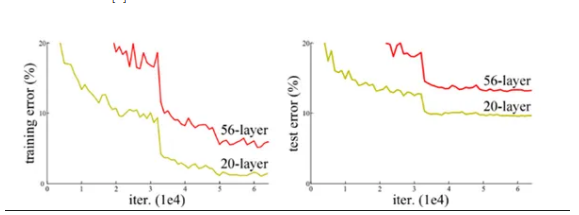
\includegraphics[width=5\textwidth, height=5cm, keepaspectratio]{RESNET18.png}
    \label{fig:enter-label}
\end{figure}

\textbf{Grafikten Çıkarılan Sonuç:} Sol taraftaki grafikte eğitim hatasını, sağ taraftaki grafikte ise test hatasını görmekteyiz. Hem eğitim verisi hem de test verisi durumunda 56 katman için hata yüzdesinin 20 katmanlı bir ağdan daha fazla olduğunu görebiliriz. Bu, bir ağın üzerine daha fazla katman eklenmesiyle performansının düştüğünü gösterir. Çok derin sinir ağlarının eğitilmesi yakınsamayı engelleyen kaybolan/patlayan gradyanlar nedeniyle oldukça zordur. Teorik olarak derinliğini arttırdığımız ağda eğitim hatasının azalmasını bekleriz fakat gerçekte doğruluk doyar ve ardından hızla düşerek eğitim hatası artar. Bu ise aşırı uyum (overfitting) nedeniyle değil, daha derin modellerin optimize edilmesinin kolay olmadığını gösteren bir bozulma (degradasyon)/optimizasyon probleminden dolayı olur.
\subsection{Artık Blok (Residual Block)Nedir?}
X katman girdisini toplama işlemine taşıyan düz çizgiye artık bağlantı (veya kısayol bağlantısı) denir. Kısayol bağlantıları, bir veya daha fazla katmanı atlayan bağlantılardır. Bu sayede, bloklarla girdiler arasında kalan bağlantılar üzerinden daha hızlı yayılabilir.\cite{SuhedaCilek}
\begin{figure}[h]
    \centering
    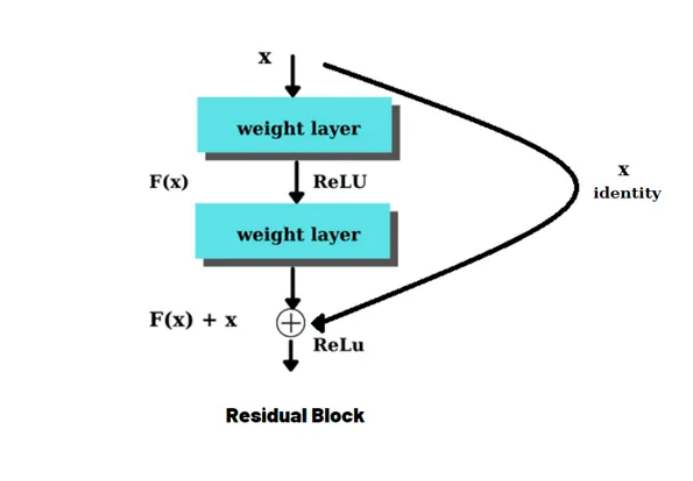
\includegraphics[width=8\textwidth, height=8cm, keepaspectratio]{artıkblok.png}
    \label{fig:enter-label}
\end{figure}

\subsection{PIL(Python Imaging Library)}
PIL (Python Imaging Library), Python için bir görüntü işleme kütüphanesidir. PIL, görüntü dosyalarını açmak, işlemek ve kaydetmek için kullanılır. PIL ile, görüntülerin boyutu değiştirilebilir, döndürülebilir, kesilebilir, birleştirilebilir ve filtreler uygulanabilir. PIL, JPEG, PNG, BMP, GIF ve diğer birçok yaygın görüntü formatını destekler. PIL görüntüsü, bir görüntüyü temsil etmek için kullanılan bir veri yapısıdır. Görüntünün piksellerini içerir ve farklı işlemler uygulamak için bir arayüz sağlar. Örneğin, bir PIL görüntüsünü gri tonlamaya dönüştürmek veya belirli bir boyuta yeniden boyutlandırmak gibi işlemler gerçekleştirilebilir.
\begin{figure}[h]
    \centering
    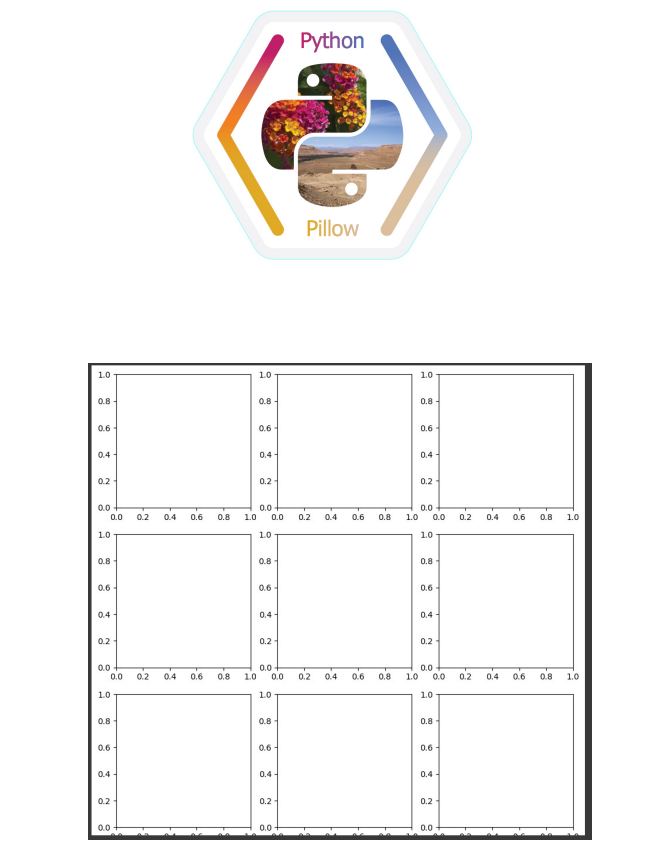
\includegraphics[width=7\textwidth, height=10cm, keepaspectratio]{pıl.png}
    \label{fig:enter-label}
\end{figure}
\subsection{ResNet}
ResNet, derin sinir ağlarının eğitimini kolaylaştırmak için geliştirilmiş bir evrişimli sinir ağı (convolutional neural network - CNN) modelidir. ResNet'in temel özelliği, ağın daha derin hale getirilmesine olanak tanıyan "skip connection" veya "shortcut connection" adı verilen bağlantıların eklenmesidir. Bu bağlantılar, bir önceki katmandan sonra gelen katmanlara doğrudan bağlanarak, gradientlerin daha düzgün bir şekilde akmasını sağlar. Bu da daha derin ağların eğitimini kolaylaştırır ve ağın performansını artırır. ResNet genellikle ImageNet veri kümesi üzerinde eğitilmiş ve çeşitli görsel tanıma görevlerinde başarılı bir şekilde kullanılmıştır. ResNet'in farklı versiyonları (örneğin, ResNet-50, ResNet-101, vb.) farklı derinliklere sahiptir ve farklı uygulamalara göre tercih edilebilir.\cite{OpenAI}
\subsection{İki Boyutlu Evrişim (2D Convolution)Nedir?}
İki boyutlu evrişim (2D convolution), dijital görüntü işleme ve işaret işleme alanlarında sıkça kullanılan bir işlemdir. Temel olarak, bir girdi görüntüsü (veya işaret) ile bir evrişim çekirdeği (kernel) arasında bir matematiksel işlem yapmayı ifade eder.

Bu işlem, her bir pikselin (veya öğenin) etrafında bir pencereyi (çekirdek) alır, bu pencereyi girdi görüntüsü üzerine yerleştirir, pencereyi ve çekirdeği eleman eleman çarparak toplar ve sonucu çıktı görüntüsüne (veya işarete) yazar. Bu işlem, girdi ile çekirdek arasında bir tür “çapraz-konvolüsyon” işlemidir.

2D evrişim genellikle görüntü işleme alanında kenar tespiti, görüntü filtreleme, özellik çıkarımı ve diğer birçok işlem için kullanılır. Örneğin, bir kenar tespit filtresi uygulamak için, kenarların görüntüdeki yoğunluk değişikliklerini vurgulayan bir çekirdek kullanılabilir.

İki boyutlu bilgiye uygulanacak olan filtrenin x ve y eksenine göre simetrisi alınır. Tüm değerler matriste eleman eleman çarpılır ve tüm değerlerin toplamı çıkış matrisinin ilgili elemanı olarak kaydedilir. Buna çapraz korelasyon ilişkisi de denir. Giriş verisi (örneğin; görüntü) tek kanallı iken bu işlem basitçe yapılabilmektedir. Ancak giriş verisi farklı formatlarda ve kanal sayısında olabilir.
\begin{figure}[h]
    \centering
    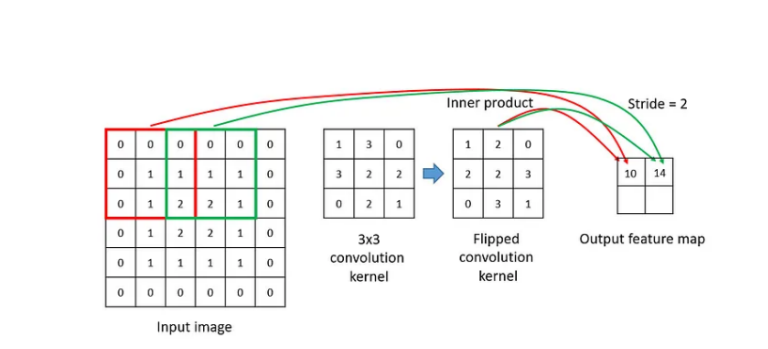
\includegraphics[width=7\textwidth, height=5cm, keepaspectratio]{2d1.png}
    \label{fig:enter-label}
\end{figure}
\subsection{RGB(Red Green Blue)}
RGB (Red, Green, Blue), renkli görüntülerin temsil edilmesinde kullanılan bir renk modelidir. Bu modelde her piksel, kırmızı (Red), yeşil (Green) ve mavi (Blue) renk kanallarının bir kombinasyonuyla oluşturulur. Her bir renk kanalı 0 ile 255 arasında değer alabilir, bu da 8 bitlik bir renk derinliğine karşılık gelir.

Her bir RGB bileşeni, 0 ile 255 arasında bir sayıyla temsil edilir. Örneğin, (255, 0, 0) kırmızıyı, (0, 255, 0) yeşili ve (0, 0, 255) maviyi temsil eder. Bu renklerin her biri farklı yoğunluklarda karıştırılarak diğer renkler elde edilebilir. Örneğin, (255, 255, 255) beyazı, (0, 0, 0) siyahı temsil eder.\cite{AyyuceKizirak}

RGB modeli, bilgisayar ekranlarında ve dijital görüntüleme cihazlarında yaygın olarak kullanılmaktadır. Renkli görüntüler, her pikseldeki RGB değerlerinin birleştirilmesiyle oluşturulur ve her bir pikselin rengini belirler.

Renkli görüntüler, Kırmızı-Yeşil-Mavi (RGB) 3 kanaldan meydana gelmektedir. Bu koşulda da evrişim işlemi 3 kanal için yapılır. Çıkış işaretinin kanal sayısı da uygulanan filtre kanalı/sayısı ile eşit olarak hesaplanır.
\begin{figure}[h]
    \centering
    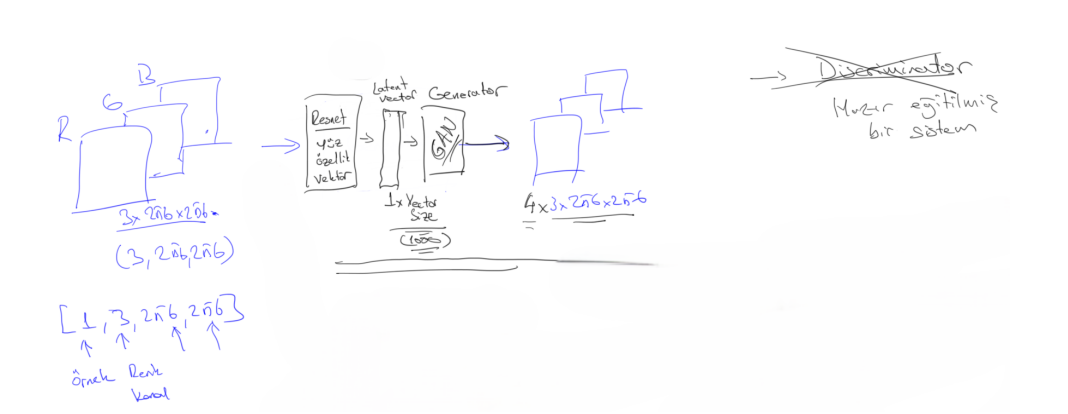
\includegraphics[width=7\textwidth, height=10cm, keepaspectratio]{resnet.png}
    \label{fig:enter-label}
\end{figure}
\begin{figure}[h]
    \centering
    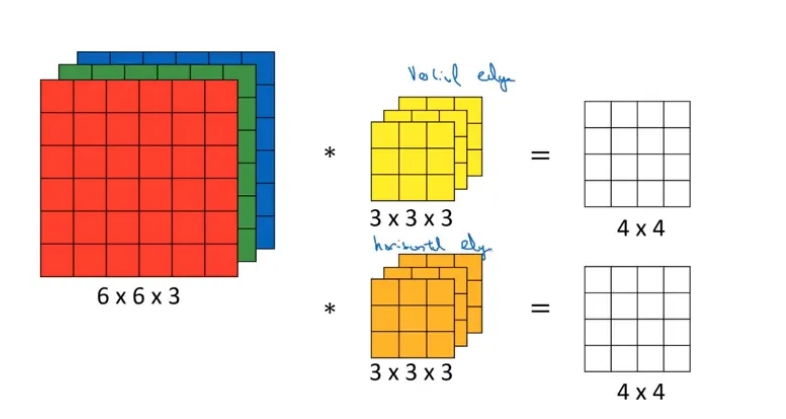
\includegraphics[width=7\textwidth, height=10cm, keepaspectratio]{rgb.png}
    \label{fig:enter-label}
\end{figure}
\clearpage
\subsection{Latent Vektör Nedir?}
Latent vektör, genellikle makine öğrenimi ve derin öğrenme alanlarında kullanılan bir terimdir. Özellikle, generatif modelleme gibi alanlarda sıkça karşımıza çıkar.

Bir generatif modelin öğrenme sürecinde, modelin girdisi olan verileri temsil etmek için kullanılan vektördür. Örneğin, GAN (Generative Adversarial Network) gibi bir modelde, latent vektör genellikle rastgele bir vektördür ve modelin öğrenme sürecinde bu vektör kullanılarak veri üretilir.

Latent vektör, genellikle modelin öğrenme sürecindeki gizli (latent) yapısını temsil eder. Bu vektör, genellikle bir önceki katmandan gelen çıktıların düzleştirilmesi veya kodlanması gibi işlemlerle elde edilir. Sonuç olarak, latent vektör, modelin öğrendiği temel özellikleri veya dağılımları içeren bir temsil olarak düşünülebilir.

Özellikle generatif modellerde, latent vektörün boyutu ve yapısı, üretilen verilerin kalitesi ve çeşitliliği üzerinde önemli bir etkiye sahip olabilir. Doğru bir latent uzay tasarımı, modelin daha iyi ve daha çeşitli veriler üretmesine yardımcı olabilir.
\begin{figure}[h]
    \centering
    \begin{minipage}{0.60\textwidth}
        \centering
        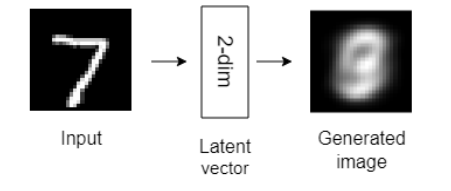
\includegraphics[width=\textwidth]{latent1.png} 
        \label{fig:resim1}
    \end{minipage}\hfill
    \begin{minipage}{0.60\textwidth}
        \centering
        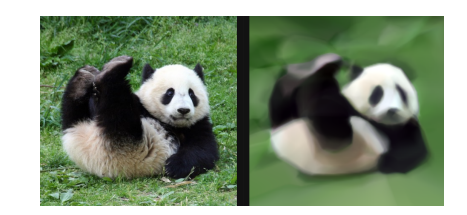
\includegraphics[width=\textwidth]{latent2.png}
        \label{fig:resim2}
    \end{minipage}
\end{figure}

\subsection{Canny Edge Detection Algorithm(Canny Kenar Tespiti Algoritması)}
Canny Edge detektörü, çok aşamalı bir algoritması olan kenar algılama işlemi için kullananılır. Canny edge, farklı görüş nesnelerinden faydalanan yapısal bilgiler elde etmek ve işlenecek veri miktarını önemli ölçüde azaltmak için kullanılan bir tekniktir. Şimdiye kadar geliştirilen kenar algılama yöntemleri arasında Canny kenar algılama algoritması, iyi ve güvenilir algılama sağlayan en katı tanımlanmış yöntemlerden biridir. Kenar algılama için üç kriteri karşılama optimalliği ve uygulama işleminin basitliği sayesinde, kenar algılama için en popüler algoritmalardan biri haline gelmiştir.
Bu tekniğin kullanımı için üç temel kriter bulunmaktadır. İlk olarak, düşük hata oranlı kenar algılama önemlidir; yani, algılama işlemi, mümkün olduğunca resimde gösterilen çok sayıda kenarı doğru bir şekilde yakalamalıdır. İkinci olarak, operatör tarafından algılanan kenar noktaları, kenarın merkezinde doğru bir şekilde konumlanmalıdır; bu, algılama sürecinin kenarların gerçek konumlarına mümkün olduğunca yakın olması gerektiği anlamına gelir. Son olarak, görüntüdeki belirli bir kenar yalnızca bir kez işaretlenmelidir ve mümkün olduğunda görüntü paraziti yanlış   kenarlar oluşturmamalıdır. Bu da algılama sürecinin gereksiz tekrarlanan kenarları tespit etme yeteneği ile ilgilidir. Bu kriterler, etkili bir kenar algılama tekniğinin başarılı bir şekilde uygulanması için önemlidir.
\begin{figure}[h]
    \centering
    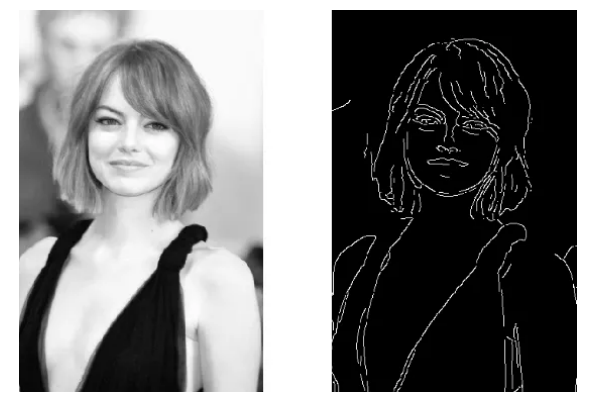
\includegraphics[width=7\textwidth, height=10cm, keepaspectratio]{canny.png}
    \label{fig:enter-label}
\end{figure}
\begin{figure}[h]
    \centering
    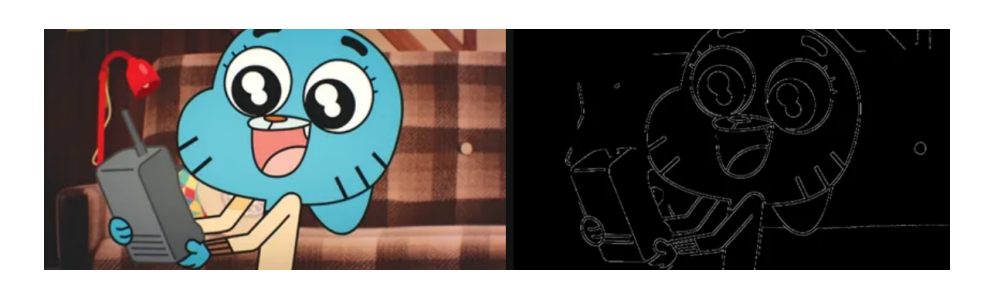
\includegraphics[width=7\textwidth, height=5cm, keepaspectratio]{e1.png}
    \label{fig:enter-label}
\end{figure}
\subsubsection{Algoritmanın İşleyiş Süreci}
\begin{center}
\tikzstyle{startstop} = [rectangle, rounded corners, minimum width=3cm, minimum height=1cm,text centered, draw=black, fill=red!30]
\tikzstyle{io} = [trapezium, trapezium left angle=70, trapezium right angle=110, minimum width=3cm, minimum height=1cm, text centered, draw=black, fill=blue!30]
\tikzstyle{process} = [rectangle, minimum width=3cm, minimum height=1cm, text centered, draw=black, fill=orange!30]
\tikzstyle{decision} = [diamond, minimum width=3cm, minimum height=1cm, text centered, draw=black, fill=green!30]
\tikzstyle{arrow} = [thick,->,>=stealth]

\begin{tikzpicture}[node distance=2cm]

\node (start) [startstop] {Başla};
\node (grayscale) [process, below of=start] {Gri Tonlama};
\node (gaussian) [process, below of=grayscale] {Gaussian Filtreleme};
\node (gradient) [process, below of=gaussian] {Kenar Şiddeti ve Yönü Hesaplama};
\node (nonmax) [process, below of=gradient] {Non-Maximum Baskılama};
\node (threshold) [process, below of=nonmax] {Eşikleme};
\node (edge) [io, below of=threshold] {Kenar Haritası};

\draw [arrow] (start) -- (grayscale);
\draw [arrow] (grayscale) -- (gaussian);
\draw [arrow] (gaussian) -- (gradient);
\draw [arrow] (gradient) -- (nonmax);
\draw [arrow] (nonmax) -- (threshold);
\draw [arrow] (threshold) -- (edge);

\end{tikzpicture}
\end{center}
\subsubsection{Gri Tonlama}
 Giriş görüntüsü gri tonlamaya dönüştürülür. Bu, her pikselin tek bir yoğunluk değeri ile temsil edildiği anlamına gelir.
 \subsubsection{Gaussian Filtreleme}
Gürültüyü gidermek için görüntüyü yumuşatmak için Gauss filtresi uygulanır. Tüm kenar algılama sonuçları görüntüdeki parazitten kolayca etkilendiğinden, neden olduğu yanlış algılamayı önlemek için paraziti filtrelemek çok önemlidir. Görüntüyü yumuşatmak için Gauss filtre çekirdeği görüntü ile birleştirilir. Bu adım, belirgin gürültünün kenar detektörü üzerindeki etkilerini azaltmak için görüntüyü hafifçe yumuşatır.
Gauss filtresinin iki boyutlu formülü şu şekildedir:

\begin{equation}
G(x, y) = \frac{1}{2\pi\sigma^2} \exp\left(-\frac{x^2 + y^2}{2\sigma^2}\right)
\end{equation}

Burada:
\begin{itemize}
    \item \( G(x, y) \): \( (x, y) \) koordinatındaki Gauss değeri.
    \item \( \sigma \): Dağılımın standart sapması.
    \item \( \exp \): Doğal logaritmanın tabanı olan \( e \)'nin üssü fonksiyonu.
\end{itemize}

Örneğin, \(\sigma = 1\) için bir 3x3 Gauss çekirdeği şu şekildedir:

\begin{equation}
G = \frac{1}{16} \begin{bmatrix}
1 & 2 & 1 \\
2 & 4 & 2 \\
1 & 2 & 1 
\end{bmatrix}
\end{equation}
\subsubsection{Kenar Şiddeti ve Yönü Hesaplama}
Görüntüdeki kenar şiddeti ve yönü hesaplanır. Bu adımda, her pikselin kenar şiddeti ve yönü, görüntüdeki yoğunluk değişikliklerinden türetilir.
\subsubsection{Non-Maximum Baskılama}
Bu adımda, kenar pikselleri çevresindeki piksellerle karşılaştırılır ve sadece lokal maksimum değerlere sahip olanlar korunur. Bu, ince kenarları korumaya ve diğer gereksiz kenarları kaldırmaya yardımcı olur.
\subsubsection{Eşikleme}
Kenar pikselleri eşik değerleriyle karşılaştırılır. Eşik değerinden büyük olan kenar pikselleri kabul edilirken, küçük olanlar reddedilir. Bu, güçlü kenarları korurken zayıf kenarları filtreler.
\subsubsection{Kenar Haritası }
Son adımda, eşiklenmiş kenar pikselleri kullanılarak kenar haritası oluşturulur. Bu, orijinal görüntünün sadece kenarlarını içeren bir görüntüdür.
\subsection{HairGAN Projesinde Kullanılan Canny Algoritması Kodu}
\begin{lstlisting}

def plot_generated_images_with_hair_detection(generator, epoch, examples=10, dim=(1, 10), figsize=(10, 1)):
    noise = np.random.normal(0, 1, (examples, 100))
    generated_images = generator.predict(noise)
    generated_images = (generated_images + 1) / 2 

    plt.figure(figsize=figsize)
    for i in range(examples):
        img = (generated_images[i] * 255).astype(np.uint8)
        gray_img = cv2.cvtColor(img, cv2.COLOR_RGB2GRAY)
        edges = cv2.Canny(gray_img, threshold1=50, threshold2=100)   
        img[edges != 0] = [255, 0, 0]  

        plt.subplot(dim[0], dim[1], i+1)
        plt.imshow(img, interpolation='bilinear')
        plt.axis('off')
    plt.tight_layout()
    plt.savefig(f"gan_generated_image_with_hair_detection_epoch_{epoch+1}.png")
    plt.show()

\end{lstlisting}
Bu fonksiyon, gray img üzerinde kenarları tespit eder. threshold1 ve threshold2 parametreleri, düşük ve yüksek eşik değerleridir ve kenar tespiti için kullanılacak eşik seviyelerini belirler.
\begin{figure}[h]
    \centering
    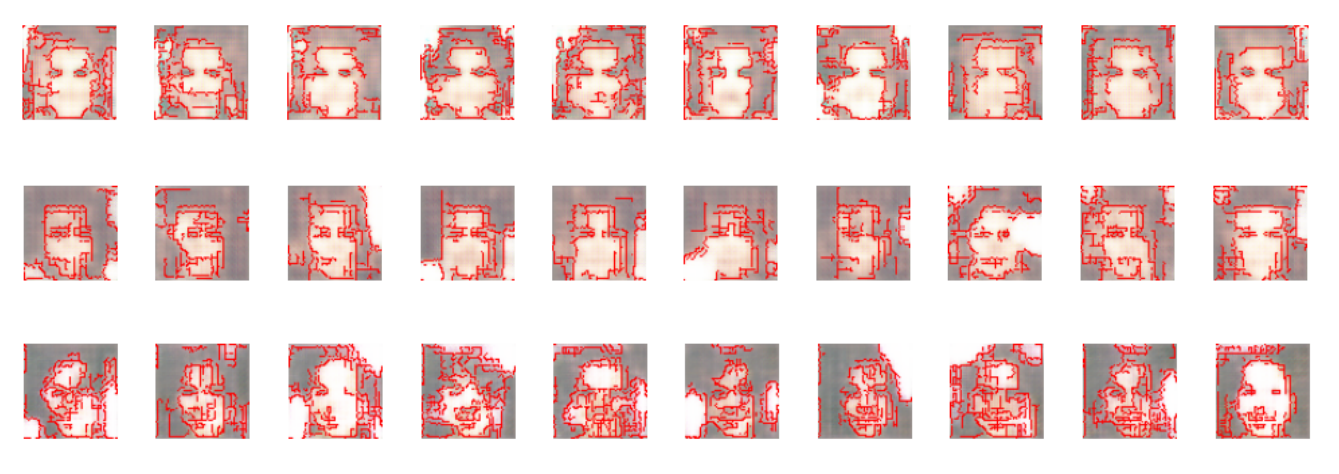
\includegraphics[width=7\textwidth, height=5cm, keepaspectratio]{canny1.png}
    \label{fig:enter-label}
\end{figure}
\newpage
\section{Literatür İncelemesi}
Generative Adversarial Networks (GAN'lar), Ian Goodfellow ve diğerleri tarafından 2014 yılında tanıtılmıştır. Bu model, bir üretici ve bir ayırt edici ağdan oluşur ve bu iki ağ arasında rekabet yoluyla gerçekçi verilerin üretilmesini sağlar. GAN'lar, derin öğrenme alanında önemli bir ilgi odağı olmuş ve birçok alanda uygulanmıştır.\cite{OpenAI}

GAN teknolojisinin gelişimiyle birlikte, birçok GAN varyasyonu ortaya çıkmıştır. Bu varyasyonlar, özellikle GAN eğitimini stabilize etmek, daha gerçekçi görüntüler üretmek veya belirli koşullara göre veri üretmek gibi belirli problemleri çözmek için tasarlanmıştır. Derin evrişimli GAN'lar (DCGAN), Conditional GAN'lar (CGAN), Wasserstein GAN'lar (WGAN), ve daha birçok varyasyon, GAN teknolojisinin gelişimine katkıda bulunmuştur.

GAN'lar, birçok alanda kullanılabilir. Görüntü üretimi, veri artırma, stil transferi, yüz ve saç stilinin oluşturulması, oyun geliştirme ve daha birçok uygulama alanında GAN teknolojisi başarıyla kullanılmıştır. Özellikle, derin öğrenme tekniklerinin ve bilgisayar grafiklerinin ilerlemesiyle birlikte, GAN'lar daha gerçekçi ve etkileyici sonuçlar elde etmekte giderek daha başarılı olmuştur.

Son yıllarda, GAN'lar özellikle yaratıcı içeriklerin üretilmesinde büyük bir rol oynamıştır. Sanat, eğlence, moda ve diğer yaratıcı endüstrilerde, GAN teknolojisi ile üretilen içerikler önemli bir etki yaratmıştır. Örneğin, yüz ve saç stilleri oluşturma gibi konularda yapılan çalışmalar, gerçekçi ve etkileyici sonuçlar elde etmiştir. Ayrıca, GAN teknolojisi, veri artırma ve sentetik veri üretimi gibi alanlarda da büyük önem taşımaktadır. Sınırlı veriyle çalışılan durumlarda, GAN'lar yeni ve çeşitli veri örneklerinin sentezlenmesine olanak tanır ve modelin genelleme yeteneğini artırabilir.

Tüm bu nedenlerden dolayı, GAN teknolojisinin geniş bir yelpazede kullanılması ve sürekli olarak geliştirilmesi, derin öğrenme ve yapay zeka alanında önemli bir araştırma ve geliştirme alanı olarak kalmaya devam edecektir.
\subsection{GAN Varyasyonları}
\begin{enumerate}[label=\textbf{\arabic*.}, leftmargin=*]
    \item \textbf{Original GAN:} Generative Adversarial Networks'in (GAN'ların) orijinal formu. Bir üretici ve bir ayırt edici ağdan oluşur ve bu iki ağ arasında rekabet yoluyla gerçekçi verilerin üretilmesini sağlar.
    
    \item \textbf{DCGAN (Deep Convolutional GAN):} Derin evrişimli ağları (CNN'ler) kullanarak daha istikrarlı ve yüksek çözünürlüklü görüntüler üretmek için GAN modelini geliştirir.
    
    \item \textbf{WGAN (Wasserstein GAN):} GAN eğitimindeki instabilite sorunlarını çözmek için bir yaklaşım sunar. Eğitim sırasında üretilen gradyanların normu üzerinde bir kısıtlama getirir ve daha istikrarlı sonuçlar elde etmeyi amaçlar.
    
    \item \textbf{CGAN (Conditional GAN):} Belirli koşullar altında özel veri üretmek için GAN modelini genişletir. Belirli bir sınıfa ait olan verilerin üretilmesini sağlar ve çeşitli uygulama alanlarında kullanılabilir.
    
    \item \textbf{CycleGAN:} Çift yönlü görüntü dönüşümü için bir GAN modelidir. İki farklı görüntü veri kümesi arasında dönüşüm yapmak için döngü tutarlılığına dayalı bir kayıp fonksiyonu kullanır.
\end{enumerate}
\subsection{GAN'ların Güncel Uygulamaları}
\begin{enumerate}[label=\textbf{\arabic*.}, leftmargin=*]
\item\textbf{Yüz ve Saç Stilleri Oluşturma:} GAN'lar, farklı yüz ve saç stillerini oluşturmak için kullanılır. Özellikle saç rengi ve kesimi gibi özelliklerde gerçekçi sonuçlar elde etmek mümkündür.

\item\textbf{Stil Transferi}: GAN'lar, bir sanat eserinin tarzını başka bir görüntüye aktarmak için kullanılabilir. Bu, farklı sanat tarzlarının sentezlenmesi veya özgün görüntünün stilize edilmesi için uygulanabilir.

\item\textbf{Veri Arttırma:} Sınırlı veriye sahip problemlerde, GAN'lar yeni ve çeşitli veri örneklerinin üretilmesine yardımcı olabilir. Bu, özellikle derin öğrenme modellerinin genelleme yeteneğini artırmak için önemlidir.

\item\textbf{Oyun Geliştirme:} GAN'lar, oyun geliştirme alanında kullanılabilir. Özellikle arka plan veya karakter oluşturma gibi görevlerde GAN'lar başarılı sonuçlar verebilir.

\item \textbf{Medikal Görüntü İşleme: }Tıbbi görüntüleme alanında, GAN'lar hastalıkların teşhisinde veya görüntü segmentasyonunda kullanılabilir. Gerçekçi tıbbi görüntülerin üretilmesi, eğitim verilerinin çeşitlendirilmesi ve model performansının artırılması için önemlidir.
\end{enumerate}
\subsection{GAN'ların Zorlukları ve Gelecekteki Yönelimler}
\begin{enumerate}[label=\textbf{\arabic*.}, leftmargin=*]
\item\textbf{Eğitim Stabilitesi:} GAN'ların eğitimi genellikle zorlu ve istikrarsız olabilir. Özellikle modellerin dengesini korumak ve patlayan/gradyanların önüne geçmek için çeşitli teknikler geliştirilmektedir.

\item\textbf{Moda Aşırı Uyum (Overfitting):} GAN'lar, eğitim verisine aşırı uyum sağlama eğilimindedir. Bu, eğitim verilerine çok iyi uyum sağlayan ancak genelleme yapmakta zorlanan modellerin oluşturulmasına yol açabilir.

\item\textbf{Hiperparametre Ayarı:} GAN'ların başarılı bir şekilde eğitilmesi için birçok hiperparametrenin doğru şekilde ayarlanması gereklidir. Bu, uzun süreli deneme yanılma süreçlerini gerektirebilir.

\item\textbf{Gelecekteki Yönelimler:} GAN teknolojisinin gelecekteki gelişimi, daha stabil eğitim tekniklerinin geliştirilmesi ve çeşitli uygulama alanlarında daha etkili kullanımı üzerine odaklanabilir. Ayrıca, daha karmaşık ve gerçekçi sonuçlar için GAN'ların mimari ve eğitim süreçlerinin iyileştirilmesi beklenmektedir.
\end{enumerate}
\subsection{GAN'ların Etik ve Güvenlik İlişkileri}
\begin{enumerate}[label=\textbf{\arabic*.}, leftmargin=*]
\item\textbf{Etik Sorunlar: }GAN'ların kullanımı, etik sorunları gündeme getirebilir. Özellikle sahte içerik üretme ve gerçeklikten ayırma konusunda ortaya çıkabilecek sorunlar düşünülmelidir. Bu, özellikle manipülatif amaçlar için kullanıldığında önemli hale gelir.

\item\textbf{Güvenlik Açıkları: }GAN'lar, veri setlerindeki örüntüleri öğrenerek tahminlerde bulunurken, yanlış verilerle yanıltılabilir. Bu, güvenlik açıklarına yol açabilir ve kötü niyetli kullanımlara zemin hazırlayabilir.

\item \textbf{Veri Mahremiyeti:} GAN'lar, gerçekçi veriler üretme yetenekleri nedeniyle veri mahremiyeti konusunda endişelere yol açabilir. Özellikle kişisel verilerin kullanımında dikkatli olunmalıdır.

\item\textbf{Çözüm Yolları:} Etik ve güvenlik konularıyla başa çıkmak için, GAN'ların kullanımını düzenleyen yasal ve etik kuralların oluşturulması önemlidir. Ayrıca, güvenlik açıklarını tespit etmek ve önlemek için teknik çözümler geliştirilmelidir.

\item\textbf{Gelecekteki Adımlar:} GAN'ların etik ve güvenlik açılarıyla ilgili araştırmaların devam etmesi ve bu teknolojinin adil ve güvenli bir şekilde kullanılmasını sağlamak için önlemlerin alınması gereklidir. Yapay zeka etiği ve güvenliği konusunda daha fazla farkındalık ve çalışma yapılması beklenmektedir.
\end{enumerate}
\section{Yöntem}
Projede CelebA veri seti kullanıldı.GAN projelerinde elimizde ne kadar çok veri olursa modelimizin öğrenmesi daha kolay olur ve overfitting(aşırı uyum) riskini azaltmış oluruz.Saç projesi için daha çok yüz görüntülerine ihtiyacımız oldu bu yüzden CelebA veri seti kullanışlıydı.
CelebA'nın kullanılma sebeplerine daha detaylı bakacak olursak :
\begin{table}[ht]
\centering
\begin{adjustbox}{max width=\textwidth}
\begin{tabular}{|p{4cm}|p{10cm}|}
\hline
\textbf{Neden} & \textbf{Açıklama} \\
\hline
Geniş Kapsam ve Çeşitlilik & CelebA veri seti, 202.599 yüz görüntüsü içermektedir. Bu geniş kapsam, makine öğrenimi ve derin öğrenme modellerinin daha çeşitli ve genelleştirilebilir sonuçlar üretmesine olanak tanır. \\
\hline
Zengin Etiket Bilgisi & Her bir görüntü için 40'tan fazla yüz özellik etiketi (örneğin, gülümseme, gözlük, sakal, saç rengi vb.) içerir. Bu, çeşitli yüz özelliklerini ve ifadelerini analiz etme ve modelleme açısından büyük avantaj sağlar. \\
\hline
Kaliteli ve Çözünürlüklü Görüntüler & Veri setindeki görüntüler yüksek kalitededir ve yüz detaylarını açıkça göstermektedir. Bu, yüz özelliklerinin ve ifadelerinin daha doğru bir şekilde tespit edilmesine yardımcı olur. \\
\hline
Standartlaştırılmış ve Yaygın Kullanım & CelebA veri seti, bilgisayarla görme ve yüz tanıma araştırmalarında yaygın olarak kullanılan bir veri setidir. Bu, literatürdeki diğer çalışmalarla karşılaştırma yapmayı ve sonuçları değerlendirmeyi kolaylaştırır. \\
\hline
Erişilebilirlik ve Kullanım Kolaylığı & CelebA veri seti, Kaggle gibi platformlardan kolayca erişilebilir ve indirilebilir. Bu, veri hazırlama sürecini hızlandırır ve kolaylaştırır. \\
\hline
Eğitim ve Test İçin Uygun & Veri seti, eğitim ve test işlemleri için ayrılmış örnekler içerir. Bu, model performansını doğru bir şekilde değerlendirmeye yardımcı olur. \\
\hline
\end{tabular}
\end{adjustbox}
\caption{CelebA Veri Setinin Tercih Edilme Nedenleri}
\label{tab:celeba_reasons}
\end{table}

\subsection{CelebA Veri Setinin Etiketlenmiş Verilerinin İncelenmesi}
Aşağıdaki tablo, CelebA veri setindeki çeşitli özelliklerin etiketlerini (Örneğin, Gülümseme, Genç, Yaşlı, Siyah Saçlı vb.) içeren ilk beş görüntünün etiketlerini gösterir. Her satır bir görüntüyü temsil eder ve her sütun bir özelliği (attributu) temsil eder. Değerler -1 (özellik yok) ve 1 (özellik var) olarak belirtilmiştir.

\begin{table}[ht]
\centering
\begin{adjustbox}{max width=\textwidth}
\begin{tabular}{lrrrrrrrrrrrrrrrrr}
\toprule
\textbf{image\_id} & \textbf{5\_o\_Clock\_Shadow} & \textbf{Arched\_Eyebrows} & \textbf{Attractive} & \textbf{Bags\_Under\_Eyes} & \textbf{Bald} & \textbf{Bangs} & \textbf{Big\_Lips} & \textbf{Big\_Nose} & \textbf{Black\_Hair} & \textbf{Sideburns} & \textbf{Smiling} & \textbf{Straight\_Hair} & \textbf{Wavy\_Hair} & \textbf{Wearing\_Earrings} & \textbf{Wearing\_Hat} & \textbf{Wearing\_Lipstick} & \textbf{Wearing\_Necklace} & \textbf{Wearing\_Necktie} & \textbf{Young} \\
\midrule
000001.jpg & -1 & 1 & 1 & -1 & -1 & -1 & -1 & -1 & -1 & -1 & 1 & 1 & -1 & 1 & -1 & 1 & -1 & -1 & 1 \\
000002.jpg & -1 & -1 & -1 & 1 & -1 & -1 & -1 & 1 & -1 & -1 & 1 & -1 & -1 & -1 & -1 & -1 & -1 & -1 & 1 \\
000003.jpg & -1 & -1 & -1 & -1 & -1 & -1 & 1 & -1 & -1 & -1 & -1 & -1 & 1 & -1 & -1 & -1 & -1 & -1 & 1 \\
000004.jpg & -1 & -1 & 1 & -1 & -1 & -1 & -1 & -1 & -1 & -1 & -1 & 1 & -1 & 1 & -1 & 1 & 1 & -1 & 1 \\
000005.jpg & -1 & 1 & 1 & -1 & -1 & -1 & 1 & -1 & -1 & -1 & -1 & -1 & -1 & -1 & -1 & 1 & -1 & -1 & 1 \\
\bottomrule
\end{tabular}
\end{adjustbox}
\caption{CelebA Veri Setindeki İlk 5 Görsel}
\label{tab:celeba_first5}
\end{table}
\newpage
\begin{figure}[h]
    \centering
    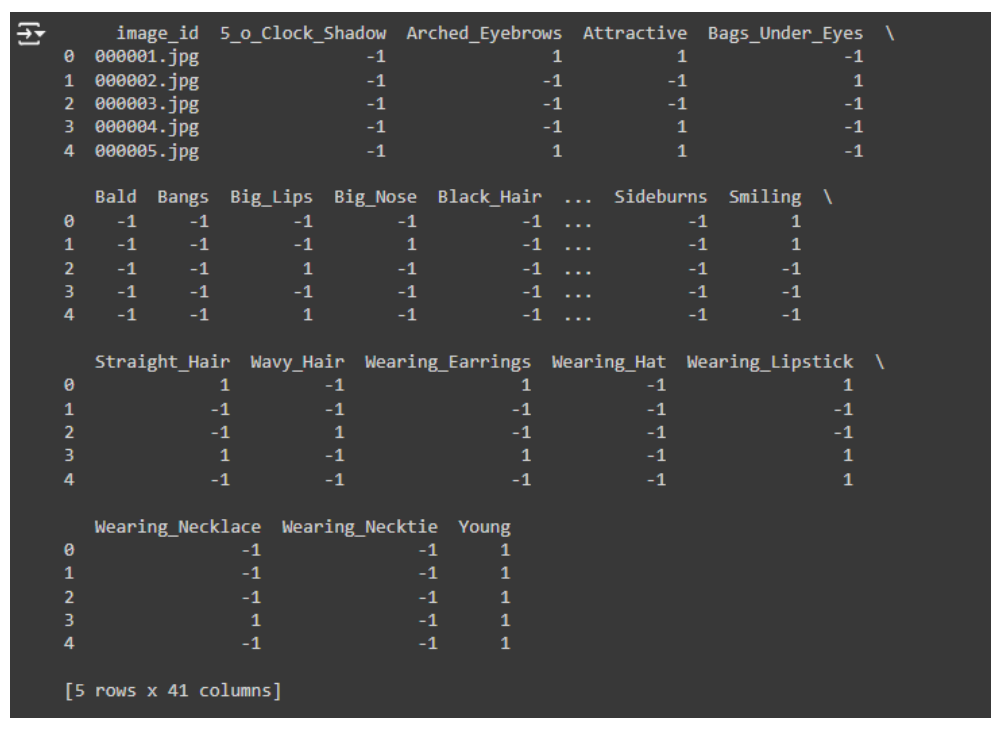
\includegraphics[width=7\textwidth, height=10cm, keepaspectratio]{rsnt.png}
    \label{fig:enter-label}
\end{figure}
\subsection{CelebA Veri Seti Kullanarak Yapılan Eğitim Sonuçları}
Model eğitimi GAN'larda çok uzun sürdü ve fazla emek istedi.Epoch arttırma ,batch size boyutunu değiştirme,steps per epoch arttırıp azaltma gibi yöntemler sayesinde en sonunda çözünürlüğü daha iyi olan görseller üretildi.En başta yapılan çalışmalarda karıncalanma,blur gibi faktörler proje sürecini epey uzattı.
\newline

\begin{figure}[H]
    \centering
    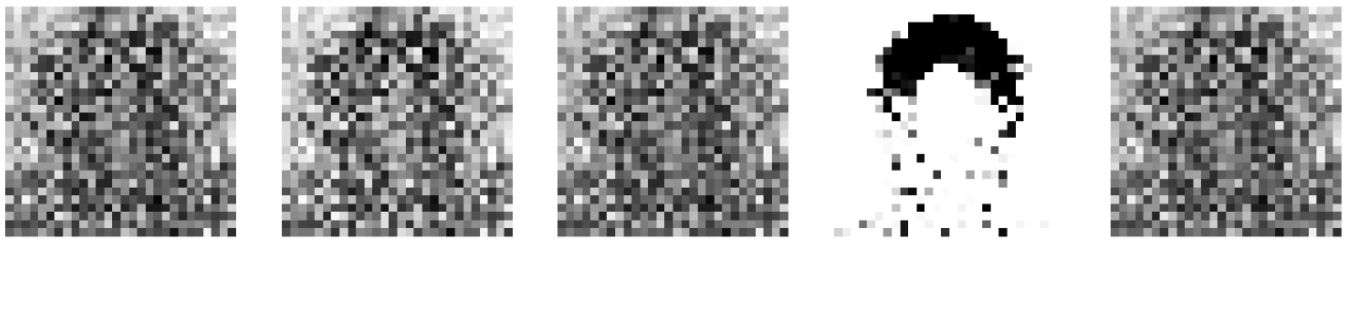
\includegraphics[width=1\textwidth, height=3cm, keepaspectratio]{1.png}
    \label{fig:enter-label}
\end{figure}
\begin{figure}[H]
    \centering
    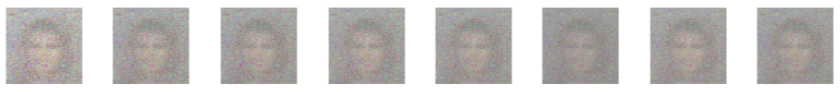
\includegraphics[width=1\textwidth, height=3cm, keepaspectratio]{2.png}
    \label{fig:enter-label}
\end{figure}
\begin{figure}[H]
    \centering
    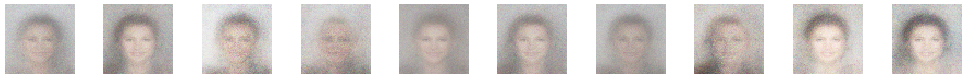
\includegraphics[width=1\textwidth, height=3cm, keepaspectratio]{4.png}
    \label{fig:enter-label}
\end{figure}
\begin{figure}[H]
    \centering
    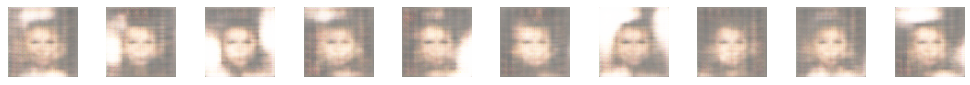
\includegraphics[width=1\textwidth, height=3cm, keepaspectratio]{5.png}
    \label{fig:enter-label}
\end{figure}
\begin{figure}[H]
    \centering
    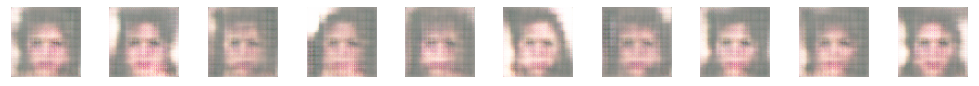
\includegraphics[width=1\textwidth, height=3cm, keepaspectratio]{6.png}
    \label{fig:enter-label}
\end{figure}
\begin{figure}[h]
    \centering
    \begin{minipage}{0.45\textwidth}
        \centering
        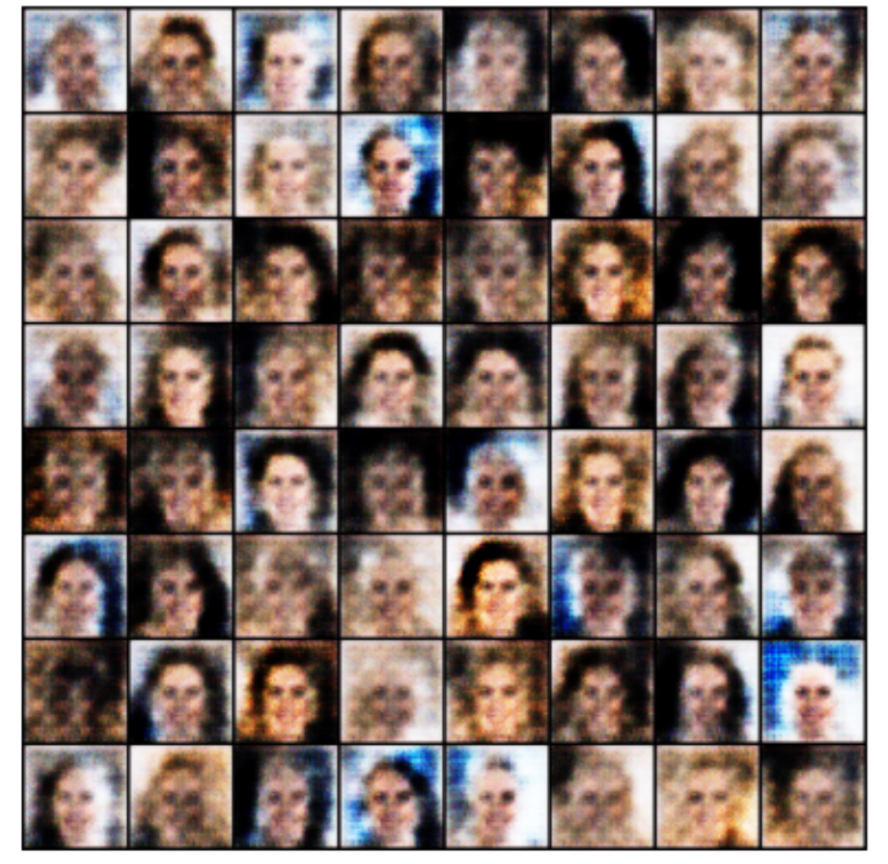
\includegraphics[width=\textwidth]{7.png} 
        \label{fig:resim1}
    \end{minipage}\hfill
    \begin{minipage}{0.45\textwidth}
        \centering
        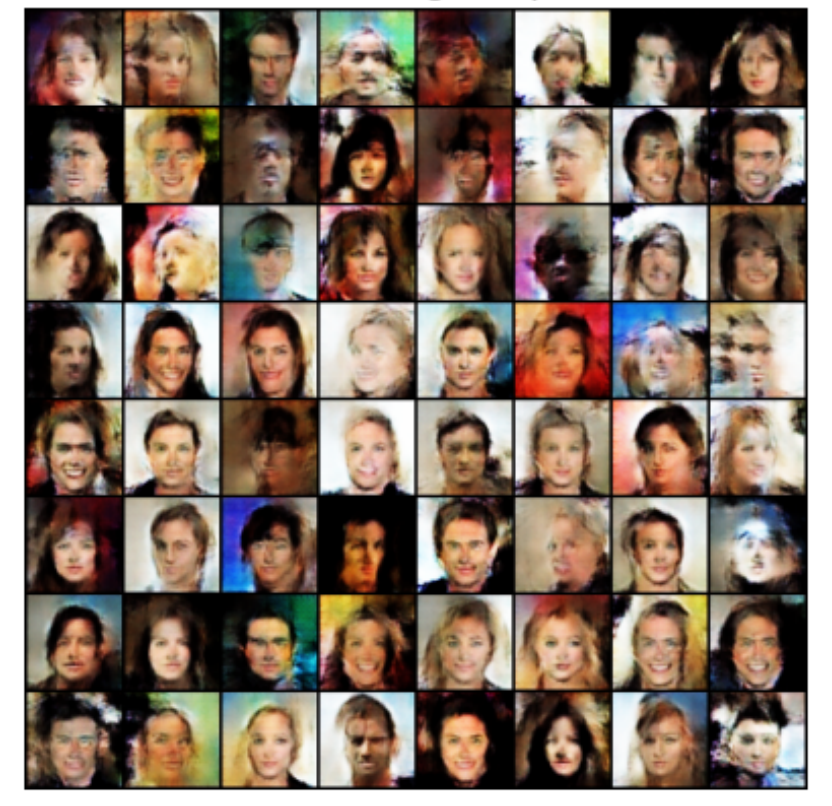
\includegraphics[width=\textwidth]{8.png}
        \label{fig:resim2}
    \end{minipage}
\end{figure}
\begin{figure}[h]
    \centering
    \begin{minipage}{0.45\textwidth}
        \centering
        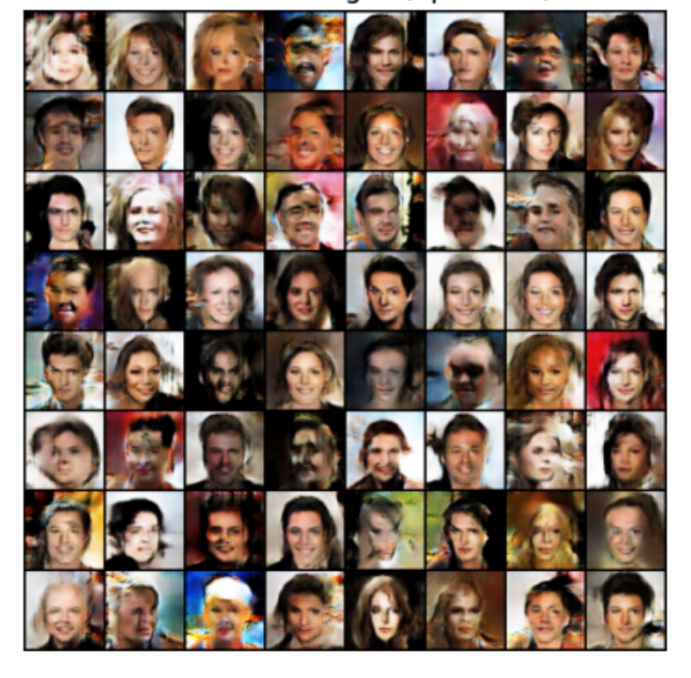
\includegraphics[width=\textwidth]{15.png} 
        \label{fig:resim1}
    \end{minipage}\hfill
    \begin{minipage}{0.45\textwidth}
        \centering
        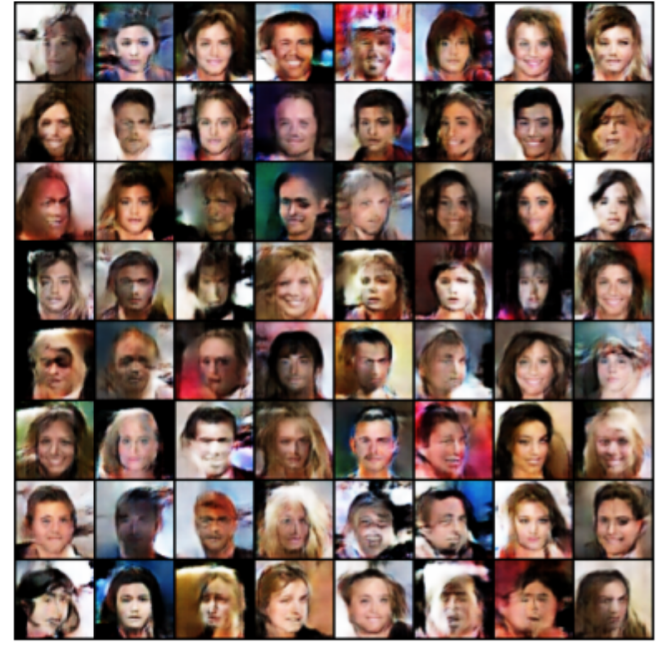
\includegraphics[width=\textwidth]{16.png}
        \label{fig:resim2}
    \end{minipage}
\end{figure}

\clearpage
\section{Sonuçlar ve Tartışma}


\subsection{Sonuçlar}
Bu çalışmada, GAN (Generative Adversarial Network) mimarisi kullanarak yüz görüntüleri oluşturma üzerine odaklandık ve Hair GAN projesinin ilk aşamasını tamamladık. Eğitim sürecinde CelebA veri seti kullanılarak GAN modelimizi eğittik. Modelimizin yüzlerin genel hatlarını doğru bir şekilde yakaladığını ve çeşitli yüz ifadeleri üretebildiğini gözlemledik.

\textbf{Başarımlar:}
\begin{itemize}
    \item \textbf{Yüz Hatları:} GAN modelimiz, yüz hatlarını genel olarak başarılı bir şekilde oluşturmuştur. Bu, modelin öğrenme kapasitesinin ve veri setinin kalitesinin bir göstergesidir.
    \item \textbf{Çeşitlilik:} Üretilen yüzler arasında çeşitli ifadeler ve farklı yüz tipleri gözlemlenmiştir, bu da modelin çeşitliliği öğrenme yeteneğini göstermektedir.
\end{itemize}

\textbf{Eksiklikler:}
\begin{itemize}
    \item \textbf{Detay Kalitesi:} Üretilen yüz görüntülerinin detay seviyesinde bazı eksiklikler bulunmaktadır. Özellikle göz, burun ve ağız gibi yüz detayları, modelin daha fazla iyileştirilmesi gerektiğini göstermektedir.
    \item \textbf{Gürültü:} Bazı görüntülerde hala belirgin miktarda gürültü ve bozulma mevcuttur, bu da modelin daha uzun süre eğitilmesi veya farklı bir mimariyle iyileştirilmesi gerektiğini göstermektedir.
\end{itemize}

\subsection{Yorumlar}
Elde edilen sonuçlar, GAN modelimizin yüz görüntülerini üretme yeteneğini başarılı bir şekilde ortaya koymaktadır. Ancak, sonuçların tam anlamıyla tatmin edici olmadığını ve daha ileri iyileştirmeler yapılması gerektiğini gözlemledik.

\textbf{Güçlü Yönler:}
\begin{itemize}
    \item \textbf{Model Performansı:} Model, yüz hatlarını ve genel yapıyı başarılı bir şekilde öğrenmiştir. Bu, modelin temel işlevini yerine getirebildiğini göstermektedir.
    \item \textbf{Çeşitli Görüntüler:} Model, çeşitli yüz ifadeleri ve yüz tipleri oluşturabilmiştir, bu da veri setinin çeşitliliği ve modelin öğrenme kapasitesi açısından olumlu bir göstergedir.
\end{itemize}

\textbf{Zayıf Yönler:}
\begin{itemize}
    \item \textbf{Detay Eksikliği:} Üretilen yüzlerdeki detay eksikliği, modelin daha karmaşık ve yüksek çözünürlüklü görüntüler oluşturma yeteneğinin sınırlı olduğunu göstermektedir.
    \item \textbf{Gürültü ve Bozulma:} Bazı görüntülerde görülen gürültü ve bozulmalar, modelin daha fazla optimizasyon gerektirdiğini göstermektedir. Bu, veri setinin kalitesi ve modelin eğitim süreci ile doğrudan ilişkilidir.
\end{itemize}

\subsection{Gelecek Çalışmalar İçin Öneriler}
Bu çalışmanın bir sonraki aşaması, yüz oluşturma sürecine saç eklemektir. Saç bölgelerinin doğru bir şekilde tanımlanması ve saç stillerinin gerçekçi bir şekilde oluşturulması için Hair GAN modelini daha da geliştirmemiz gerekmektedir. Gelecek çalışmalarda, aşağıdaki adımların izlenmesi önerilmektedir:

\begin{enumerate}
    \item \textbf{Saç Verilerinin Eklenmesi:} CelebA veri setine ek olarak, farklı saç stillerini içeren veri setlerinin kullanılması. Bu, modelin çeşitli saç stillerini öğrenmesini ve oluşturmasını sağlayacaktır. Özellikle düz, kıvırcık ve dalgalı saçların gerçekçi bir şekilde oluşturulması için bu tür verilerin eklenmesi gerekmektedir.
    \item \textbf{Modelin İyileştirilmesi:} Modelin mimarisinin daha karmaşık hale getirilmesi ve hiperparametre optimizasyonu ile performansının artırılması. Örneğin, daha derin ve geniş bir ağ yapısı kullanarak, modelin öğrenme kapasitesi artırılabilir.
    \item \textbf{Veri Ön İşleme:} Saç ve yüz bölgelerinin daha net bir şekilde ayrılması için veri ön işleme adımlarının iyileştirilmesi. Bu, özellikle saç çizgisinin ve saç stilinin doğru bir şekilde belirlenmesi için önemlidir.
    \item \textbf{Saç Oluşturma Algoritmaları:} Saç stilini belirleme ve gerçekçi saç yapısı oluşturma için yeni algoritmaların ve tekniklerin uygulanması. Örneğin, stil transferi veya dikkat (attention) mekanizmaları kullanarak saç yapısının daha gerçekçi ve çeşitli olması sağlanabilir.
    \item \textbf{Kalite Değerlendirmesi:} Üretilen görüntülerin kalitesini değerlendirmek ve iyileştirmek için yeni metriklerin kullanılması. Görüntü kalitesini artırmak için PSNR (Peak Signal-to-Noise Ratio) veya SSIM (Structural Similarity Index) gibi metrikler kullanılabilir.
\end{enumerate}

\textbf{Önerilen Çalışma Adımları:}
\begin{itemize}
    \item \textbf{Veri Setinin Genişletilmesi:} Çeşitli saç stillerini içeren daha geniş bir veri seti oluşturulması. Bu, modelin daha fazla çeşidi öğrenmesini sağlayacaktır.
    \item \textbf{Model Mimarisinin Yeniden Tasarımı:} Daha derin ve geniş bir ağ yapısının kullanılması. Bu, modelin daha karmaşık yapıları öğrenmesine yardımcı olacaktır.
    \item \textbf{Eğitim Sürecinin İyileştirilmesi:} Hiperparametre optimizasyonu, veri artırma (augmentation) teknikleri ve daha uzun eğitim süreleri kullanarak modelin performansının artırılması.
    \item \textbf{Sonuçların Değerlendirilmesi:} Üretilen görüntülerin kalitesini objektif metriklerle değerlendirmek ve kullanıcı geri bildirimleriyle iyileştirmeler yapmak.
\end{itemize}

Bu öneriler doğrultusunda, Hair GAN projesi kapsamındaki yüz ve saç oluşturma süreçleri daha başarılı ve gerçekçi sonuçlar verecektir. Gelecek çalışmalar, bu projeyi daha ileriye taşıyacak ve daha kaliteli, gerçekçi görüntüler elde edilmesini sağlayacaktır.
\section{Kaynakça}
\printbibliography
\section{Teşekkür}
Bu yapay zeka projesinin gerçekleştirilmesinde emeği geçen ve desteklerini esirgemeyen herkese en içten teşekkürlerimi sunarım.

Öncelikle, projem boyunca beni yönlendiren, değerli bilgileri ve tavsiyeleriyle çalışmama katkıda bulunan değerli hocam Emre GÜNGÖR'e  şükranlarımı sunarım. Onun rehberliği ve desteği olmadan bu proje mümkün olmazdı.

Ayrıca, gerekli veri setlerini ve kaynakları sağlayarak çalışmamı kolaylaştıran Kaggle platformuna  teşekkür ederim. Bu çalışmanın her aşamasında yanımda olan ve moral desteği veren arkadaşlarıma da minnettarım.

Son olarak, Google Colab platformunu kullanarak çalışmalarımı gerçekleştirmemi sağlayan Google'a teşekkür ederim. Bu platform sayesinde projelerimi daha etkili ve verimli bir şekilde gerçekleştirebildim.
\end{document}





